%!TEX root = ../../head.tex

\chapter{Übung}

\section{Einführung}
timo.schick@tu-dresden.de

\subsection{}
\begin{enumerate}
	\item Sterntopologie: Ein zentrales Element(Sternkoppler), jeder 				Rechner benötigt eine Leitung zu Sternkoppler \(\to\) 5
	\item Jeder mit Jedem \(= 4+3+2+1=10\)
	\item
	\begin{enumerate}
		\item \(l(n)= n\) bei Sterntopologie
		\item \(l(n) = \sum ... = (n*(n-1))/2\) bei vollvermaschter 					Topologie
	\end{enumerate}
	\item
	\begin{enumerate}
		\item LAN
		\begin{itemize}
			\item Reichweite: ~10m
			\item Reaktionszeit: niedrig
			\item Datenrate: hoch
			\item Topologien: Sterntopologie
		\end{itemize}
		\item MAN
		\begin{itemize}
			\item Reichweite: ~10km
			\item Reaktionszeit: mittel
			\item Datenrate: mittel
			\item Topologien: hierarchische Topologie
		\end{itemize}
		\item WAN
		\begin{itemize}
			\item Reichweite: ~100km - ~10.000km
			\item Reaktionszeit: hoch
			\item Datenrate: niedrig
			\item Topologien: Vollvermaschte Topologie
		\end{itemize}
	\end{enumerate}
\end{enumerate}

\subsection{}
\begin{enumerate}
	\item Dienst und Protokoll
	\begin{itemize}
		\item siehe Musterlösung
	\end{itemize}
	\item OSI Schichtenmodell
	\begin{itemize}
		\item Schichtenmodell siehe Folie 1.8ff
		\item Protokoll:
		\begin{itemize}
			\item ist eine Sprache zur horizontalen Kommunikation 							zwischen Prozessen derselben Schicht auf verschiedenen 						Hosts
		\end{itemize}
		\item Dienst
		\begin{itemize}
			\item dient der vertikalen Kommunikation zwischen zwei 							Schichten auf einem Host
		\end{itemize}
		\item Aufteilung des Bitstroms: Schicht 2 Sicherungsschicht
		\item Ende-zu-Ende Kommunkation: Schicht 4 Transportschicht
		\item Wegewahl: Schicht 3 Vermittlungsschicht
	\end{itemize}
	\item keine inhaltliche Bearbeitung, sondern nur 								Informationsweiterleitung
\end{enumerate}

\subsection{}
\begin{enumerate}
	\item
	\begin{itemize}
		\item siehe Folie 1.15; 
		\item Initiator (Prozess A), ...
		\item Responder (Prozess B), ...
	\end{itemize}
	\item
	\begin{enumerate}
		\item Zustände bestimmen
		\begin{itemize}
			\item idle
			\item connected
			\item prepare(Initiator)
			\item prepare(Responder)
		\end{itemize}
		\item Übergänge bestimmen (Knoten, Pfad, Knoten)
		\begin{itemize}
			\item (idle, conReq, prep(Init))
			\item (idle, ConInd, prep(Resp))
			\item (prep(Resp), conRsp, connected)
			\item (prep(Init), conCnf, connected)
			\item (connected, dataRep/dataInd, connected) 
			\item (prep(Resp)/prep(Init)/connected, disRep/disInd, idle)
		\end{itemize}
	\end{enumerate}
	\item
	\begin{enumerate}
		\item Ablaufdiagramm
		\begin{itemize}
			\item c1) + zeitlicher Ablauf
			\item c2) - es werden n Diagramme benötigt
			\item c3) - 
		\end{itemize}
		\item Zustandsdiagramm
		\begin{itemize}
			\item c1) - 
			\item c2) + alle Abläufe in einem Diagramm darstellbar
			\item c3) + 
		\end{itemize}
	\end{enumerate}
\end{enumerate}

\subsection{}
\begin{enumerate}
	\item siehe Folie 1.10
	\begin{enumerate}
		\item \(PDU(N)=SDU(N-1)\)
		\item \(IDU(N)=ICI(N)+SDU(N)\)
	\end{enumerate}
	\item Seitenaufruf: http://www.heise.de/software
	\begin{enumerate}
		\item httpRequest
		\begin{enumerate}
			\item  GET/software/http/1.1
			\item Host: www.heise.de
		\end{enumerate}
		\item ICI 
		\begin{enumerate}
			\item ip: 193.99.144.85 port:80
		\end{enumerate}
		\item SDU
		\begin{enumerate}
			\item  GET/software/http/1.1
			\item Host: www.heise.de
		\end{enumerate}
		\item IDU
		\begin{enumerate}
			\item ICI
			\item SDU
		\end{enumerate}
		\item TCP-PDU
		\begin{enumerate}
			\item src:80, dest:80,...
			\item SDU
			\item Data
		\end{enumerate}
	\end{enumerate}
	\item	
	\begin{align*}		
		b_{0}&=125\frac{\text{Mbit}}{\text{s}}\\
		b_{1}&=b_{0}\cdot0,8\\
		b_{2}&=b_{1}\frac{(55+99)0,01}2\\
		b_{3}&=b_{2}\frac{(57+99)0,01}2\\
		b_{4}&=b_{3}\frac{(23+99)0,01}2=36,4\frac{\text{Mbit}}							{\text{s}}\\
		b_{4}&=b_{goodput}\\
		b_{extra}&=b_{2}\frac{(23+99)0,01}2=46,7\frac{\text{Mbit}}						{\text{s}}
	\end{align*}
\end{enumerate}

\section{Bitübertragungsschicht}
\subsection{Nyquist-Theorem}
\begin{enumerate}
	\item 
	\begin{itemize}
		\item Bandbreite B [Hz]
		\item Signalrauschabstand SNR
		\item Abschneidefrequenzen in niedrigen Bereichen \(\to\) Differenz = Bandbreite
		\item Signalstufen S [1], digitaler Signal: \(S = 2\)
		\item Signalrate SR [Hz]
		\item Bitrate b \([\frac{\text{Bit}}{\text{s}}]\)
	\end{itemize}
	\(b = SR \cdot ld(S)\)
	\begin{itemize}
		\item Nyquist 1 (rauschfrei) \(b < 2\cdot B\cdot ld(2)\)
		\item Nyquist 2 (verrauscht) \(b < B \cdot ld(1+SNR) \)
		\item \(SNR_{dB} = 10 \cdot log_{10}(SNR)\)
	\end{itemize}
	Informationsgehalt \(I = ld(16) = 4 \text{ [Bit]f}\)\\
	Signalrate \(SR = \frac{b}{ld(S)} = \frac{9600 \frac{\text{ Bit}}{\text{s}}}{4 \text{ [Bit]}} \)
	\item
	\begin{align*}
	&SNR_{dB} = 12 \text{dB} \\ &SNR = 10^{\frac{SNR_{dB}}{10}} = 15 \\ &B > \frac{b}{(d(1+SNR))} = \frac{9600\frac{\text{Bit}}{\text{s}}}{ld(1+15)} = 2400 \text{Hz}
	\end{align*}
	\item 
	\begin{displaymath}
		B > 963 Hz \to B > 1200 Hz \text{Nyquist 1}
	\end{displaymath}
\end{enumerate}
\subsection{Pulsecodemodulation}
\begin{enumerate}
	\item
	\begin{itemize}
		\item PCM: analoges Signal \(\to\) Tiefpass \((f_{g}) \to \) Abtastung (zeitdiskret, \((f_{a})\)) \\ \(\to\) Quantisierung (wertdiskret)
		\item \(f_{a} > 2 f_{g}\)
	\end{itemize}
	gegeben: 
	\begin{align*}
		&B = 60 \text{ kHz} \\
		&QS = 1024 \\
		&S = 2
	\end{align*}
	gesucht:
	\begin{align*}
		b &< 2\cdot B \cdot ld(S) \\
		&= 2 \cdot 60\text{ kHz} \cdot 1\text{ [Bit]} \\
		&= \frac{120\text{ kBit}}{\text{s}}\\ \\
		f_{a} &= \frac{b}{(d(QS))}	\\
		&= \frac{b}{10\text{ [Bit]}} \\
		&= 12 \text{ kHz} \\
		f_{g} &< \frac{f_{a}}{2} \\
		&= 6 \text{ kHz}
	\end{align*}
	
	\item
	\begin{itemize}
		\item 8 Bit: leises Hintergrundrauschen
		\item 4 Bit: starkes Rauschen
		\item 1 Bit: extremes Rauschen
	\end{itemize}
\end{enumerate}
\subsection{Modulation}
\begin{enumerate}
	\item Tabelle zeichnen siehe VL
	\begin{enumerate}
		\item Amplitudenmodulation
		\item Frequenzmodulation
		\item Phasenmodulation
	\end{enumerate}
	\item 
	\begin{itemize}
		\item Realisierungsaufwand
		\begin{enumerate}
			\item sehr gut
			\item gut
			\item schlecht
		\end{enumerate}
		\item Störsicherheit
		\begin{enumerate}
			\item schlecht
			\item gut
			\item sehr gut
		\end{enumerate}
	\end{itemize}
\end{enumerate}
\subsection{Leitungskodierung}
\begin{enumerate}
	\item Leitungskodierung: \\Anpassung des Datenstroms an das eingesetzte Übertragungsmedium \\ 
	Ziel:
	\begin{itemize}
		\item Erkennung von Leitungsunterbrechungen
		\item Synchronisation (\(\to\) Takt)
	\end{itemize}
	\item einfacher Manchesterkodierung
	\begin{itemize}
		\item Leitungskode (Takt kann herausgelesen werden, Leitungen können unterbrochen werden)
		\item jedes Bit in zwei Intervalle teilen
		\item 0 \(\to\) low, high
		\item 1 \(\to\) high, low
	\end{itemize}
	\item siehe b)\\
	Übertragungsrate = \(\frac{1}{2}\) Signalrate
\end{enumerate}
\subsection{Multiplex}
\begin{enumerate}
	\item siehe Musterlösung
	\begin{itemize}
		\item synchrones Zeitmultiplex
		\begin{itemize}
			\item feste Zeitschlitze - Taktung nötig
			\item fester Zeitabschnitt für jeden Sender
			\item Zuordnung zu virtuellem Kanal durch Position im Übertragungskanal
		\end{itemize}
		\item asynchrones Zeitmultiplex
		\begin{itemize}
			\item feste Zeitschlitze - Taktung nötig
			\item Senden nach Bedarf
			\item Channel Identifier für Zuordnung zu virtuellem Kanal
		\end{itemize}
	\end{itemize}
	\item gegeben:
	\begin{align*}
		&B_{\text{Gesamt}} = 49 \text{ MHz} \\
		&B_{\text{Abstand}} = 1,5 \text{ MHz} \\
		&B_{\text{Kanal}} = 5,5 \text{ MHz}
	\end{align*}
	gesucht: Anzahl n der möglichen Fernsehkanäle:
	\begin{align*}
		&49 \text{ MHz} = 5,5 \text{ MHz} \cdot n + 1,5 \text{ MHz} \cdot (n - 1) \\
		&49\text{ MHz} = (5,5+1,5)\text{ MHz} \cdot n - 1,5 \text{ MHz} \\
		&50,5 = 7n \\
		&n = \frac{50,5}{7} = 7,21
	\end{align*}
	\(\to\) Es können 7 Kanäle angeboten werden.
\end{enumerate} 

\section{Netztechnologien 1}
\subsection{Ethernet}
\begin{enumerate}
	\item CSMA/CD
	\begin{enumerate}
		\item \(t_0\): A beginnt ein Frame zu senden
		\item \(t_0 + \tau - \epsilon\) B beginnt ein Frame zu senden
		\item \(t_0 + \tau \) B erkennt Kollision
		\item \(t_0 + \tau - \epsilon + \tau\) A erkennt die Kollision
	\end{enumerate}
	\(\Rightarrow t_s > 2\tau \) mit \(t_s\) Sendezeit für ein Frame
	\begin{align*}
	\tau &= \frac{d_{ges}}{v_{phy}}\\
	&= \frac{\text{|Repeater| }+1 \cdot d}{v_{phy}}\\
	&= \frac{5\cdot 500 \text{ m}}{\frac{200000 \text{km}}{s}}\\
	&= 12,5 \mu s\\
	&\rightsquigarrow 2\tau = 25 \mu s\\
	&\text{Sendezeit} = \frac{\text{Rahmenlänge}}{Bitrate}\\
	t_s &= \frac{F}{b}\\
	F &= t_s \cdot b > 2\tau \cdot b\\
	&= 25\mu s \cdot 10 \frac{\text{MBit}}{s}\\
	&= 250 \text{Bit}\\
	\end{align*}
	\item Ethernet Flow Control
	Switches kümmern sih um die Behandlung von potentiellen Kollisionen EFC dient ... siehe Lösungen
\end{enumerate}
\subsection{Switches}
	|Präambel (8)|Ziel (6)|Quelle (6)|Typ/Size (2)|\\Daten (1500)|CRC (4)|Interframe Gap (12)| \(\rightsquigarrow \) () in Byte
\begin{enumerate}
	\item Store-and-Foreward Switches \\
	\(t_s \text{ und } t_V\) werden vernachlässigt
	\begin{align*}
	&t_s + t_F + t_V + t_s + t_F\\
	t_F &= \frac{SL +F}{b} = \frac{(8+1518)\cdot 8\text{Bit}}{100 \cdot 10^6 \frac{\text{Bit}}{s}}\\
	&= 122,08 \mu s \\
	t_{ges} &= 4 t_F = 488,32 \mu s
	\end{align*}
	\item Virtual-Cut-Through Switches
	\begin{align*}
	&t_s + t_H + t_s + t_F\\
	t_{ges} &= 3t_H + t_F \\
	&= 122,08 \mu s + 3 \cdot \frac{14 \cdot 8\text{ Bit}}{100 \cdot 10^6 \frac{\text{Bit}}{s}}\\
	&= 122,08 \mu s + 3 \cdot 1,12 \mu s \\
	&= 125,44 \mu s
	\end{align*}
\end{enumerate}
\subsection{Transparent Bridges}
\begin{enumerate}
	\item Wegewahltabellen siehe Lösungen
	\item Bridge Informationen: \\
	X|Y : \\
	X = kommt von welchem Rechner, \\
	Y = kommt an welchem Port an
	\item Probleme 
	\begin{itemize}
		\item bei Zyklen (Pakete werden im Kreis weitergereicht
	\end{itemize}
	\item Spanning Tree Protocol
	siehe Lösungen
\end{enumerate}
\subsection{802.11 WLAN}
\begin{enumerate}
\item 
Wkt., dass ein Bit falsch ist: 
\begin{align*}
&e_{\text{Bit}} = 3 \cdot 10^{-6}
\end{align*}
Wkt., dass ein Bit richtig ist: 
\begin{align*}
&p_{\text{Bit}} = 1- e_{\text{Bit}}
\end{align*}
Rahmen mit 1500 Byte Größe:
\begin{align*}
&p_{Frame} = p_{Bit} \cdot \ldots \cdot p_{Bit} = (p_Bit)^{1500 \cdot 8} \\
&= (1-3\cdot 10^{-6})^{12000} = 0,96464 \\
e_{\text{Frame}} = 1-p_{Frame} = 0,035\\
\to \text{im Mittel 3,5 prozent der Frames fehlerhaft.}
\end{align*}
\item 
\begin{align*}
p_{Frame} &= (p_{Bit})^{(64\cdot 8)} = 0,99847\\
\to e_{Frame} &= 0,00153
\end{align*}
\end{enumerate}

\section{Netztechnologien 2}
\subsection{WiMax}
siehe Musterlösung
\subsection{RPR}
\begin{enumerate}
	\item Zeichnen Sie eine Topologie mit einem RPR Router pro Universität und den entsprechenden Ringlet-Verbindungen
	\item Abb.: \ref{img:RPR1}
	\begin{figure}
		\centering
		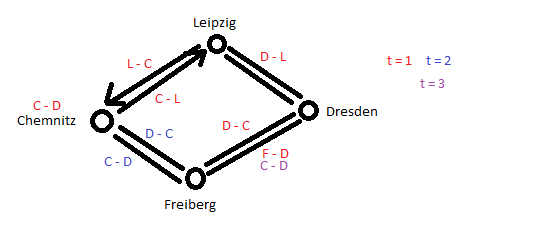
\includegraphics[width = 12cm]{./Rechnernetze/Images/4_2ab.png}
		\caption{RPR a) und b)}
		\label{img:RPR1}
	\end{figure}
	\item Abb.: \ref{img:RPR2}
	\begin{figure}
		\centering
		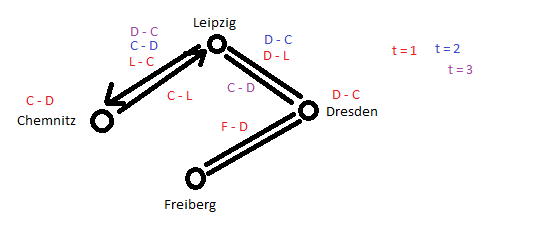
\includegraphics[width = 12cm]{./Rechnernetze/Images/4_2c.png}
		\caption{RPR c)}
		\label{img:RPR2}
	\end{figure}
\end{enumerate}
\subsection{Carrier Ethernet}
\begin{enumerate}
	\item Abb.: \ref{img:Netzaufbau}
	\begin{figure}
		\centering
		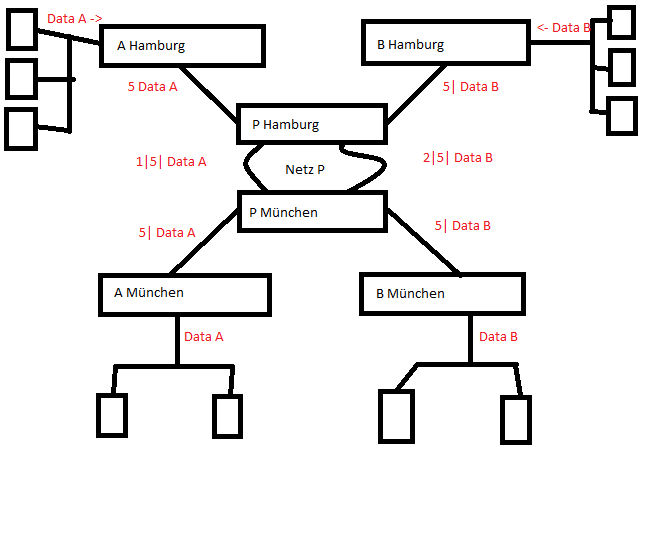
\includegraphics[width = 12cm]{./Rechnernetze/Images/4_3ab.png}
		\caption{Netzaufbau}
		\label{img:Netzaufbau}
	\end{figure}
	\item Abb.: \ref{img:Netzaufbau}
	\item Abb.: \ref{img:EthernetHeaderfeld}
	\begin{figure}
		\centering
		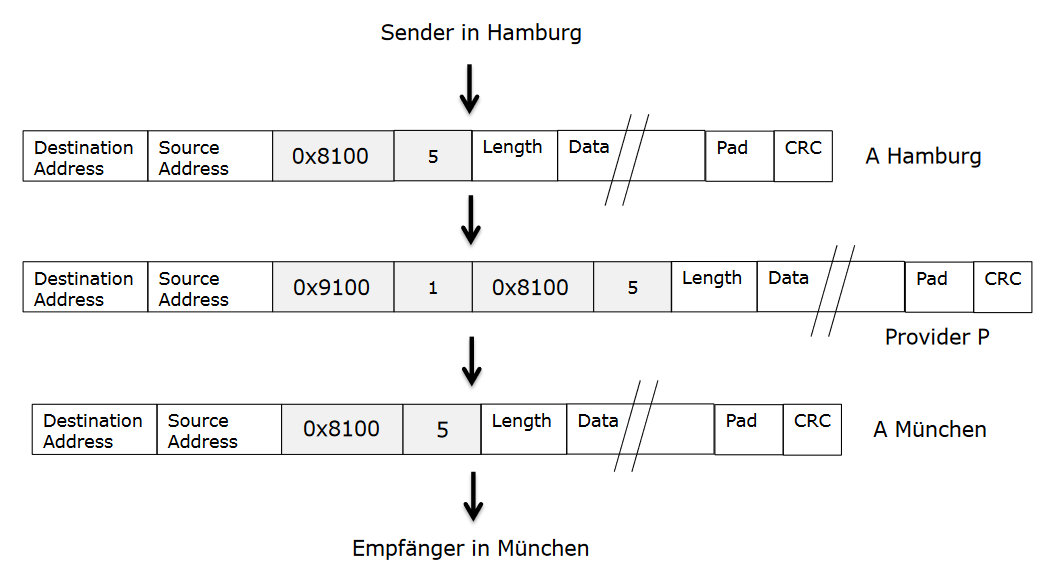
\includegraphics[width = 16cm]{./Rechnernetze/Images/4_3c.png}
		\caption{Ethernet Headerfeld}
		\label{img:EthernetHeaderfeld}
	\end{figure}
\end{enumerate}
\subsection{MPLS}
zu Abb.: \ref{img:MPLS} \\
\begin{tabularx}{\textwidth}{|X|X|X|X|r|}
\hline
	&\textbf{IN}	 	&\textbf{DEST}			&\textbf{OUT} &\\
\hline
\multirow{6}{*}{\textbf{SF}}
	&(1,-)	&134.5.0.0/16	&(3,1) &a)\\ 
	&(1,-)	&230.3.0.0/16	&(2,2) &a)\\
	&(2,7)	&*				&(1,-)	&c)\\
	&(3,10)	&*				&(1,-)	&c)\\
	&(1,-)	&134.5.42.0/24	&(2,11) &d)\\
	&(2,14)	&*				&(1,-)	&d)\\
\hline
\multirow{2}{*}{\textbf{H}}
	&(1,1)	&	&(3,4) &a) \\
	&(3,9)	&	&(1,10)&c) \\
\hline
\multirow{2}{*}{\textbf{W}}
	&(1,4)	&	&(3,5) &a)\\
	&(3,8)	&	&(1,)	&c)\\
\hline
\multirow{2}{*}{\textbf{C}}
	&(1,2)	&	&(2,3) &a)\\
	&(2,6)	&	&(1,7)	&c)\\
	&(1,11)	&	&(2,12)	&d)\\
	&(2,13)	&	&(1,14)	&d)\\

\hline
\multirow{2}{*}{\textbf{NY}} 
	&(2,5)	&*		&(3,-) &a)\\
	&(1,3)	&*		&(4,-) &a)\\
	&(4,-)	&217.8.0.0/16	&(1,6) &c) \\
	&(3,-)	&217.8.0.0/16	&(2,8)	&c) \\
	&(1,12)	&*		&(3,-)	&d)\\
	&(3,-)	&217.8.42.0/24	&(1,13)&d)\\
\hline
\end{tabularx}
\begin{figure}
		\centering
		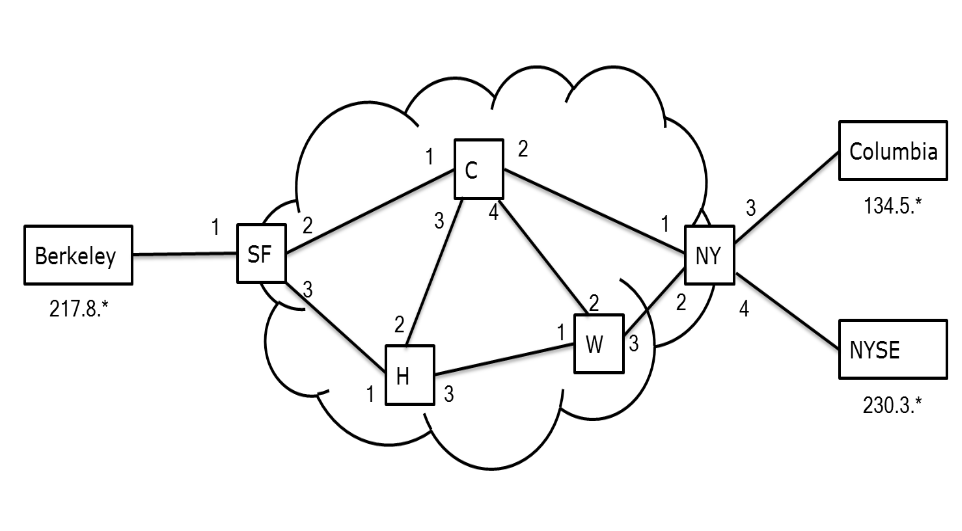
\includegraphics[width = 16cm]{./Rechnernetze/Images/4_4.png}
		\caption{MPLS-Network}
		\label{img:MPLS}
	\end{figure}
\begin{itemize}
	\item[b)] 
	\begin{tabularx}{\textwidth}{|X|X|X|}
	\hline
	Teilstrecke	&Label	&Ip-Dest \\
	\hline
	Berkeley - SF	&-	&134.5.20.217 \\
	\hline
	SF - H		&1	&134.5.20.217 \\
	\hline
	H - W		&4	&134.5.20.217\\
	\hline
	W - NY		&5	&134.5.20.217 \\
	\hline
	NY - Columbia	&-	&134.5.20.217 \\
	\hline
\end{tabularx}
\end{itemize}
\subsection{SONET/SDH und OTN}
Abb.:\ref{img:SONET}
\begin{figure}
		\centering
		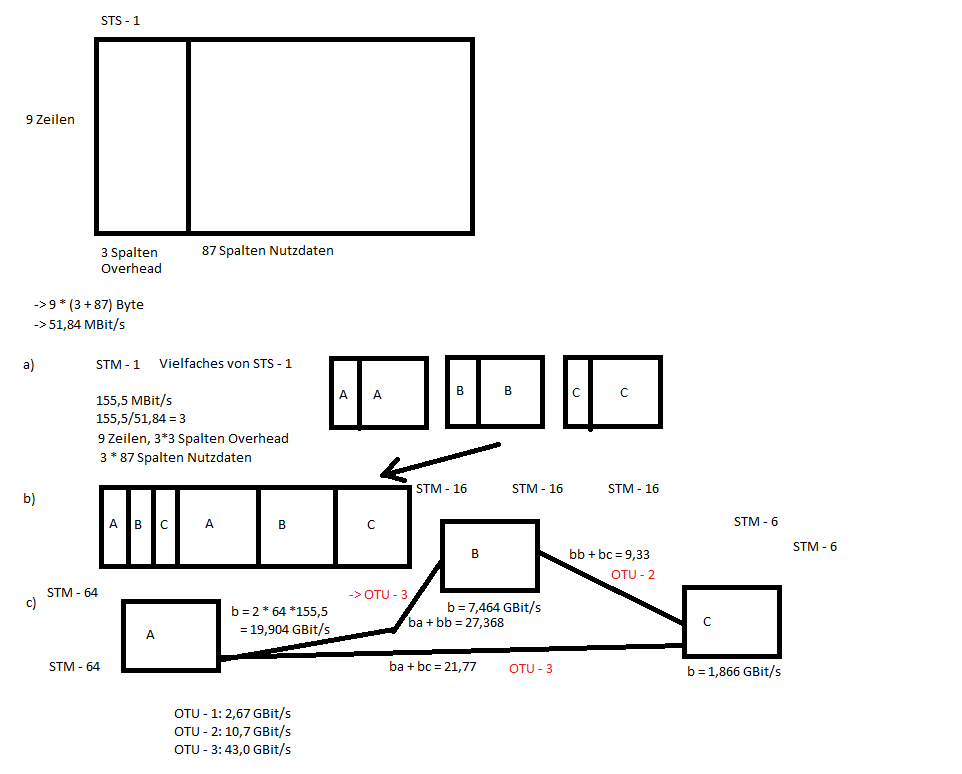
\includegraphics[width = 16cm]{./Rechnernetze/Images/4_5abc.png}
		\caption{STS - 1 und STM - N \((n \in \mathbb N)\)}
		\label{img:SONET}
\end{figure}
\section{Sicherungsschicht}
\subsection{Rahmenbildung}
\begin{enumerate}
	\item RB = 01111110\\
	RB|n Bits|RB
	\begin{itemize}
		\item T = 101 0100
		\item o = 110 1111
		\item k = 110 1011
		\item e = 110 0101
		\item n = 110 1110
	\end{itemize}
	\(\to\) 01111110 101 0100 110 1111 110 1011 \ldots 01111110
	\item Rahmenbegrenzer teil der n Bits zwischen o und k
	\item Bit-Stuffing: Jede Folge aus fünf 1en wird mit einer 0 erweitert, Empfänger löscht nach 111110 die 0.\\
	Byte-Stuffing: ESC-Sequenz: A|RB|B \(\to\) A|ESC|RB|B\\
	A|ESC|B \(\to\) A|ESC|ESC|B
\end{enumerate}
\subsection{Fehlerkorrigierende Codes}
\begin{enumerate}
	\item 
	\begin{enumerate}
		\item B
		\item C
		\item B
		\item A oder B
		\item A
	\end{enumerate}
	\item min(d(A,B),d(A,C),d(B,C)) = $  $3
	\item $ f_e = d-1 = 2$\\ $f_k = \frac{d-1}{2} = 1$
\end{enumerate}
\subsubsection{Paritätsbit}
\begin{enumerate}
	\item (Un)gerade Parität: Paritätsbit wird so gewählt, dass die Anzahl an 1en (un)gerade ist.
	\begin{enumerate}
		\item $|101100111|_1 = 6 \to $ Störung oder Par.Bit falsch berechnet
		\item $|101011100|_1 = 5 \to $ richtig übertragen oder gerade Anzahl Bitfehler
	\end{enumerate}
\end{enumerate}
\subsection{CRC}
\begin{enumerate}
\item G(x): Generatorpolynom\\
r = grad(G(x))\\
$P_D$: Datenpolynom\\
m = grad($P_D$)\\
$x^5+x^4+x^2+1 \to 110101$\\
r = 5
\begin{align*}
10100&0110100000 \div 110101 \\
11010&1\\
01110&1\\
 1101&01\\
 0011&1010\\
   11&0101\\
     &111110\\
     &110101\\
     &00101100\\
     &00110101\\
     &000110010\\
     &000110101\\
     &0000001110 = Rest \to 1010001101 01110
  \end{align*}
\item $101000110101110\div 110101 \to Rest = 0$
\item
\begin{align*}
&b = 40 kBit/s\\
&\tau = 20 ms\\
&T = t_s+ 2\tau\\
&50\% Effizienz\\
t_s &= 0,5T\\
&= 0,5(t_s + 2\tau)\\
&= 0,5 t_s + \tau\\
0,5 t_s &= \tau\\
\Rightarrow &t_s = 2 \tau\\
&\frac{F}{b} = 2\tau\\
F &= 2\tau b = 2 \cdot 20 \cdot 40 = 1600Bit
\end{align*}
\end{enumerate}
\section{Vermittlungsschicht}
\subsection{Shortest Path Algorithmus (Dijksstra-Algorithmus)}
Wähle Startknoten als permanenter und Arbeitsknoten $\to$ Wähle als nächsten Arbeitsknoten den Knoten mit dem Geringsten Pfad und setzte ihn permanent $\to$ ...
\begin{enumerate}
	\item A $\to$ F in Schritten
	\begin{itemize}
		\item permanenter Knoten A; Arbeitsknoten A
		\begin{itemize}
			\item B: (A,3), C:(A,4)
		\end{itemize}		 
		\item permanenter Knoten A,B; Arbeitsknoten B
		\begin{itemize}
			\item D: (B,8), E:(B,5)
		\end{itemize}
		\item permanenter Knoten A,B,C; Arbeitsknoten C
		\begin{itemize}
			\item D: (C,5)
		\end{itemize}
		\item permanenter Knoten A,B,C,E; Arbeitsknoten E
		\begin{itemize}
			\item F: (B,11)
		\end{itemize}
		\item permanenter Knoten A,B,C,E,D; Arbeitsknoten D
		\begin{itemize}
			\item F: (D,9)
		\end{itemize}
	\end{itemize}
	Der kürzeste Weg ist demzufolge: $A\to C\to D\to F$ mit Kosten 9. 				Tabellarisch mit Spalten Knotenvorrat(momentan erreichbare Knoten, 1.Sp: 		\{B,C\}), Arbeitsknoten (1.Sp: A), Wege (1.Sp: (AB,3) (AC,4)
	\item Es gibt nur einen Pfad $\to$ ABEF(11) muss der kürzeste Weg sein
\end{enumerate}
\subsection{Einsatz von IP: Adressen und Subnetze}
\begin{enumerate}
	\item Aufteilung der IP-Adressen in Netzanteil und Geräteanteil $\Rightarrow$ Hierarchisches Routing:
	\begin{itemize}
		\item Subnetzadressen müssen außerhalb einer Organisation nicht bekannt sein
		\item Routingtabellen werden deutlich kleiner
	\end{itemize}
	\item
	\begin{itemize}
		\item Netzanteil = IP-Adresse AND Maske
		\item Geräteanteil = IP-Adresse AND NOT Maske
		\item 129.44.0.0/\textbf{16} $\to$ Maske: 1111111111111111 0...16x...0
		\begin{align*}
			&A_1 = 129.44.0.7\\
			&M_1 = 2255.255.128.0\\
			&A_1 = 1000 0001.00101100.00000000.00000111\\
			&M_1 = 1111111111111111 1000 000000000000\\
			\to &S_1 = 1000000100101100.0000000000000000\\
			&S_1 = 129.44.0.0\\
			&X = 2^{15}-2  = 2^{\text{|Geräteanteil|}}-2 = 2^{32- \text{|Netzanteil|}}-2
		\end{align*}
		reservierte Adressen: Geräteanteil = 0 ... 0 (Netzwerk) bzw. 1 ... 1 (Broadcast)
		\begin{align*}
			&A_2 = 1000001.00101100.11100000.00001111\\
			&M_2 = 1111 1111 1111 1111 1100 0000 0000 0000\\
			&Y = 2^{14} -2
		\end{align*}
	\end{itemize}
\end{enumerate}
\subsection{}
\begin{itemize}
	\item C ist Routng-Firewall
	\item INF1 und ZIH1 sind Default-Router, INF2 und ZIH2 sind Standby-Router
\end{itemize}
\begin{enumerate}
	\item A $\to$ Router SyA $\to$ Firewall SyA $\to$ INF1 $\to$ ZIH1 $\to$ Internet $\to$ D $\to$ Internet $\to$ ZIH1 $\to$ INF1 $\to$ |A| $\to$ B
	\item	
	\begin{itemize}
	\item SyA: 141.76.40.0/22
	\item IAI: 141.76.82.0/24
	\item Firewalls: 141.76.29.32/28
	\end{itemize}
	Routing Tabellen:	
	\begin{itemize}
		\item INF1
		\begin{itemize}
			\item Typ
			\begin{itemize}
				\item C
				\item C
				\item S
				\item D
			\end{itemize}
			\item Filter
			\begin{itemize}
				\item 141.76.29.32/28
				\item 141.76.82.0/24
				\item 141.76.40.0/22
				\item 0.0.0.0/0
			\end{itemize}
			\item Ziel
			\begin{itemize}
				\item Firewalls
				\item IAI
				\item 141.76.29.33
				\item ZIH1
			\end{itemize}
		\end{itemize}
		\item Routing Firewall C
		\begin{itemize}
			\item Typ
			\begin{itemize}
				\item C
				\item D
			\end{itemize}
			\item Filter
			\begin{itemize}
				\item 141.76.40.0/22
				\item 0.0.0.0/0
			\end{itemize}
			\item Ziel
			\begin{itemize}
				\item SyA
				\item INF1
			\end{itemize}
		\end{itemize}
\end{itemize}		
\item dynamische Einträge (z.B. OSPF)
\item primär nach den Netzmasken (größte zuerst), sekundär nach IP-Adressen (kleinste zuerst) $\Rightarrow$ Longest Prefix Match
\item dynamische Routen werden auf INF2 umgeleitet
\end{enumerate}
\subsection{}
\begin{enumerate}
	\item Internet Control Message Protocol (ICMP), Type 8 (Echo(ping)request)
	\item 
	\begin{itemize}
		\item src: 192.168.1.102
		\item dst: 128.59.23.100
	\end{itemize}
	\item Ja. TimeToLive = 1 (TTL). Jeder Router verringert TTL um 1. Wenn TTL = 0, sendet Router eine ICMP Typ 11 (TTL exceeded)-Nachricht.
	\item Fragmentierung
	\begin{itemize}
		\item erstes Fragment: more fragments(1) fragement offset(0)
		\item weiteres Fragment: more fragments(1) fragment offset (>0)
		\item letztes Fragment: morefragments(0) fragment offset (>0)
		\item hier: 0/0
	\end{itemize}
	$\rightsquigarrow$ nicht fragmentiert
	\item 
	\begin{itemize}
		\item Src und Dst bleiben gleich
		\item total length, TTL, headerchecksum \textbf{können} sich ändern
		\item Identification \textbf{muss} sich ändern
	\end{itemize}
\end{enumerate}
\subsection{IPv6}
\begin{enumerate}
	\item 
	\begin{itemize}
		\item IPv4: 32-Bit-Adressen. Theoretisch $2^{32} = 4,3$ Mrd mögliche Adressen $\to$ nur ein Teil der Adressen wegen Subnetzeinteilung und reservierten Adressen nutzbar
	 	\item IPv6: 128-Bit-Adressen. Theoretisch ca $3,4 \cdot 10^{38}$ Adressen möglich
	 \end{itemize}
	 \item
	 \begin{itemize}
	 	\item Vergrößerung des Adressraums (siehe a))
	 	\item Vereinfachung Header
	 	\item Vereinfachung mobiler Netzwerkteilnahme (Mobile IP siehe Ü12)
	 	\item Implementierung von Sicherheitsmerkmalen (IPsec)
	 	\item Qualitätsmerkmale werden unterstützt (siehe Ü10)
	 \end{itemize}
	 \item Berechnungen in Netzwerkgeräten i.d.R. aus Effizienzgründen in der Hardware realisiert $\to$ Umstellung von 32 auf 128 Bit ist von der Hardware abhängig
\end{enumerate}
\section{Transportschicht}
fill siehe Tobi telegramm
\section{Netzwerkperformance}
\subsection{Ehernet-Performance}
\begin{enumerate}
	\item
	\begin{enumerate}
		\item Fast Ethernet: Fmin = 64Byte, Fmax = 1518 Byte, SL = 8Byte, IFG = 12Byte \\ Berechnung $\eta$ siehe Lösungen
		\item Gigabit Ethernet: Fmin = 512Byte, Fmax = 1518 , SL = IFG  = 8
		\begin{itemize}
			\item Padding: 8(SL) 64(F) \ldots(PAD) 8(IFG) \\ Berechnung $\eta$(Pad + F auf 512) siehe Lösungen
			\item Bursting: 8(SL) 64(F) 8(IFG) \ldots (PAD) $\to$ \ldots \\ Berechnung $\eta$ siehe Lösungen, n = 13 (aus Vorlesung)
		\end{itemize}
	\end{enumerate}
	\begin{itemize}
		\item Jumbo-Frames: $F_{max} = 8192$Byte
		\begin{align*}
			n\cdot (SL+F+IFG9)+PAD &\le 8192 \text{Byte}\\
			80n &\le 8192 - 448 = 7744\\
			n &\le 96,8 \\\rightsquigarrow n &= 96\\
			\eta_{\text{Frame}} &= \frac{n\cdot F}{n(SL+F+IFG)+PAD}\\
			&= \frac{96\cdot 64 Byte}{96(8+64+8)\text{Byte}+448\text{Byte}}\\
			&= 75,59\%
			\end{align*}
	\end{itemize}
	\item 
	\begin{itemize}
		\item F = 128 Byte
		\item PAD = (512-128)Byte = 384Byte
		\item Fast Ehernet: $\eta_{\text{Frame}}$ = 86,49\%
		\item GB Eth. + PAD: $\eta_{\text{Frame}}$ = 24,24\%
		\item GB Eth. + PAD + BURST: $\eta_{\text{Frame}}$ = 64,37\%, n = 7
		\item Jumbo Frames: $\eta_{\text{Frame}}$ = 84,71\%, n = 54
	\end{itemize}
\end{enumerate}
\subsection{Fairness}
\begin{enumerate}
	\item Fairness bezeichnet den gleichberechtigten und gleichmäßigen Zugriff aller Teilnehmer eines Netzwerkes auf die vorhandenen Ressourcen.
	\begin{itemize}
		\item unfair:
		\begin{figure}[ht]
		\centering
		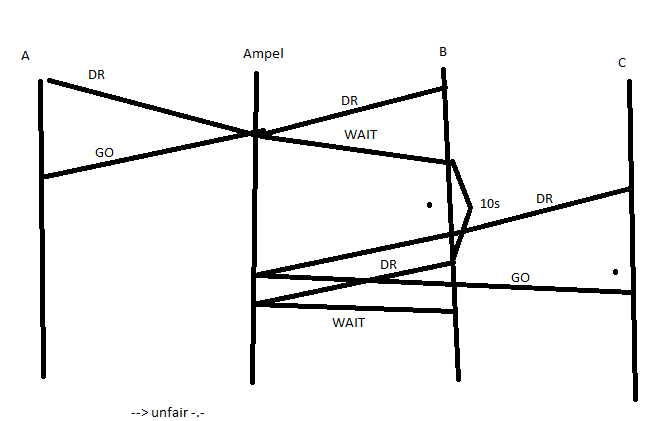
\includegraphics[width = 15cm]{./Rechnernetze/Images/8_2b.png}
		\caption{unfair}
		\label{img:unfair}
\end{figure}
\end{itemize}
		\item fair: Server vergibt Wartenummern. DriveRequest 0: Wartenummer zieehen[Wait(WN)] DriveRequest WN : Go wenn WN richtig
		\begin{figure}[ht]
		\centering
		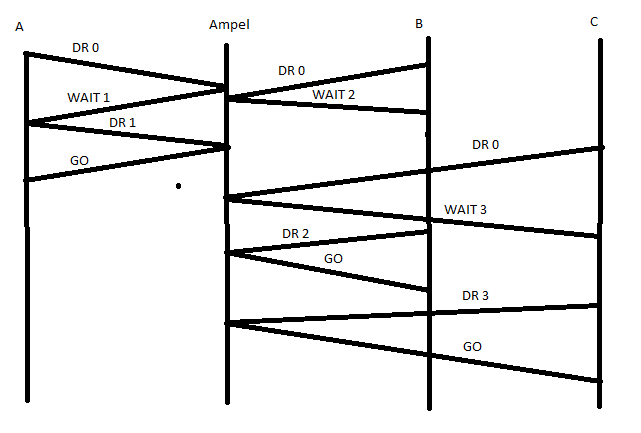
\includegraphics[width = 15cm]{./Rechnernetze/Images/8_2b2.png}
		\caption{fair}
		\label{fair}
\end{figure}
\end{enumerate}
\subsection{Überlastungsüberwachung}
\begin{enumerate}
	\item 
	\begin{itemize}
		\item Nachfrage: x1 = 6, x2 = 6,5, x3 = 12, x4 = 15, K = 30 $\to \frac{30}{4}$
		\item Runde 1: k1 = 6, k2 = 6,5, k3 = 7,5, k4 = 7,5, Ü1 = 1,5, Ü2 = 1 K = 2,5$\to \frac{2,5}{2}$
		\item Runde 2: k3 = 8,75, k4 = 8,75
	\end{itemize}
	\item $K = 16\text{, }g_{\text{ges, ungesättigt}} = \Sigma g_i k_i^* = K \cdot \frac{g_i}{g_{\text{ges, ungesättigt}}}$
	\begin{align*}
		g_{\text{ges, ungesättigt}} &= 2,5 + 4 + 0,5 + 1 = 8\\
		k_1^* &= 16 \cdot \frac{2,5}{8} = 5\\
		k_2^* &= 16 \cdot \frac{4}{8}= 8\\
		k_3^* &= 16 \cdot \frac{0,5}{8} = 1\\
		k_4^* &= 16 \cdot \frac{1}{8}= 2 \\
		\text{RUNDE 1:} &x_1 = 4, x_2 = 2, x_3 = 10, x_4 = 5 \\
		&k_1 = 4, k_2 = 2, k_3 = 1, k_4 = 2, U_1 = 1, U_2 = 6\\
		&K = U_1 + U_2 = 7\\
		&g_{\text{ges, ungesättigt}} = 0,5 + 1 = 1,5\\
		k_3^* = 7 \cdot \frac{0,5}{1,5} = 2,33\\
		k_4^* = 7 \cdot \frac{1}{1,5} = 4,67\\
		\text{RUNDE 2:} &k_3 = 3,33 k_4 = 5, U_4 = 1,67\\
		\text{RUNDE 3:} &k_3 = 5 \to k_3 \text{ ist ungesättigt}
	\end{align*}
\end{enumerate}
\subsection{Überlaststeuerung}
\begin{align*}
	&\text{Last}_\text{neu} = a \cdot \text{Last}_\text{alt} + (1-a)\cdot \text{Last}_\text{aktuell} \\ &a \ldots \text{ Anpassungsfaktor, } a = 0,3 \text{ Last}_\text{alt} = 0\\
	&\text{Last}_\text{aktuell}\\
	&1: \text{Last}_\text{neu} = 0,3 \cdot 0 + (1-0,3) \cdot 1 = 0,7\\
	&5: \text{Last}_\text{neu} = 0,3 \cdot 0,7 + 0,7 \cdot 5 = 3,71\\
	&8: \text{Last}_\text{neu} = 0,3 \cdot 3,71 + 0,7 \cdot 8 = 6,71\\
	&9: \text{Last}_\text{neu} = 0,3 \cdot 6,71 + 0,7 \cdot 9 = 8,31 \to \text{\textbf{CHOKE}}\\
	&9: \text{Last}_\text{neu} = 0,3  \cdot 8,31 + 0,7 \cdot 9 = 8,79 \to \text{\textbf{CHOKE}}\\
	&7: \text{Last}_\text{neu} = 0,3  \cdot 8,79 + 0,7 \cdot 7 = 7,54 \\
	&2: \text{Last}_\text{neu} = 0,3  \cdot 7,54 + 0,7 \cdot 2 = 3,66 \\
\end{align*}
\subsection{Leistungssteigerung}
\begin{enumerate}
	\item BDP: Anzahl an Daten (in Bit), die auf einer Leitung liegen: \\$BDP = b \cdot \tau$ 
	\begin{itemize}
		\item wird weniger gesendet, als das BDP, ist die Leitung nicht ständig belegt $\to$ Empfängerfenster $\le$ BDP
		\item Go-Back-N: bleibt eine Bestätigung aus, muss der gesamte Leitungsinhalt wiederholt werden
	\end{itemize}
	\item $v = \frac{d}{\tau} \rightsquigarrow \tau = \frac{d}{v} = \frac{4000 \text{ km}}{200000 \frac{\text{km}}{\text{s}}}$\\$BDP = b \cdot \tau =  \frac{4000 \text{ km}}{200.000 \frac{\text{km}}{\text{s}}}\cdot 1\frac{\text{GBit}}{\text{s}} = 20\text{ MBit} = 2,5 \text{MB}$  \\keine Bedeutung für die Framegröße
	\item $BDP = 2 \cdot b \cdot \tau = 2 \cdot 640\frac{GBit}{s} \frac{8000 \text{ km}}{200000 \frac{\text{km}}{\text{s}}}\\ = 51,2 GBit = 6,4 GB > 650 MB$
\end{enumerate}
\section{Internetdienste}
\subsection{Domain Name System (DNS)}
\begin{enumerate}
	\item $\underbrace{\text{www.}}_{hostname}\underbrace{\text{inf.}}_{subdomain}\underbrace{\text{tu-dresden.}}_{domain}\underbrace{\text{de}}_{top level domain}$
	\item
	\begin{enumerate}
		\item DNS Client $\leftrightarrow$ DNS Server
		\begin{itemize}
			\item Client sendet den Namen, zu dem IP benötigt wird, an seinen Default-DNS-Server
			\item Server kümmert sich um komplette Adressermittlung
			\item ermittelte Adresse wird an Client übermittelt
		\end{itemize}
		\item DNS Server $\leftrightarrow$ DNS Server
		\begin{itemize}
			\item falls IP für DNS-Server unbekannt: Weiterleitung der Anfrage an hierarchisch höheren/niedrigeren Server
		\end{itemize}
	\end{enumerate}
	\item 
	\begin{tabularx}{\textwidth}{|X|X|X|X|X|}
	\hline 
	NAME &TTL(Sek.) &CLASS &TYPE &VALUE\\
	\hline
	jupiter (relative Adressierung) & 86.400 &IN &A &117.186.1.1\\
	\hline
	jupiter & 86.400 &IN &AAAA &2001:db8:\par 85a3:8d3::1 \\
	\hline
	saturn &86.400 &IN &A & 117.186.1.2\\
	\hline
	saturn &86.400 &IN &AAAA & \ldots ::2\\
	\hline
	rn-edu.de\textbf{.} &86.400 &IN &NS &sonne\\
	\hline
	sonne &86.400 &IN &A & 117.186.1.3\\
	\hline
	sonne &86.400 &IN &A & \ldots ::3\\
	\hline
	\_ sip.\_ tcp.rn-edu.de\textbf{.} &86.400 &IN &SRV &0 0 5060 mond.\par rn-edu.de\textbf{.}\\
	\hline
	\_ sip.\_ udp.rn-edu.de\textbf{.} &86.400 &IN &SRV &0 0 5060 mond.\par rn-edu.de\textbf{.}\\
	\hline
	mond & 86.400 &IN &A&117.186.1.4\\
	\hline
	mond & 86.400 &IN &AAAA &2001: \ldots ::4\\
	\hline
	\end{tabularx}
	\begin{itemize}
	\item A = IPv4 - Adresse
	\item AAAA = IPv6-Adresse
	\item SRV = Service
	\item NS = Name Server
	\end{itemize}
\end{enumerate}
\subsection{E-Mail}
Base64: Binary-to-Text-Encoding\\
Vorgehensweise: je 3 Byte werden in 4 6-Bit-Blöcke aufgeteilt. Jeder 6-Bit-Block wird mit einem ASCII-Zeichen codiert (8 Bit). Ggf. werden Füllbytes angehängt.\\
Ausgangsgröße von 20.000 Byte (ab hier alles in Byte)\\
Anzahl 3er-Gruppen: $\frac{20000}{3} = 6666,67 \to 6667$ Gruppen\\
Anzahl Bytes (Base64): $6667 \cdot 4 = 26668$\\
Anzahl Zeilenumbrüche: $\lceil \frac{26668}{76} \rceil = 351$\\
Gesamtzahl Bytes: $26668 + 351 \cdot 2 = 27370$

\subsection{World Wide Web}
\begin{enumerate}
	\item
	\begin{enumerate}
		\item Position im HTML-Dokument feststellen
		\item Auswertung der Anweisung <a href = "http://www. \ldots " > link </a>
		\item Zielserver muss aus URL ermittelt werden\\$\to$ DNS-Anfrage (Dienst)
		\item www-Seite mittels HTTP anfordern (Protokoll)
		\item HTTP-Response auswerten, Seite darstellen
	\end{enumerate}
	\item 
	\begin{enumerate}
		\item gaia.cs.umass.edu/cs451/index.html
		\item HTTP/1.1
		\item Ja. $\to$ Connection: Keep-Alive 
		\item unbekannt
	\end{enumerate}
	\item
	\begin{enumerate}
		\item Ja. $\to$ 200 OK
		\item 12:39:45GMT
		\item 18:27:46GMT
		\item 3874
		\item <!doc \ldots 
		\item Ja. $\to$  Connection: Keep-Alive		
	\end{enumerate}
	\item 
	\begin{enumerate}
		\item Dienste: 
		\begin{itemize}
			\item OpenURL(String URL)
			\item ReceivedRessource (buffer res)
		\end{itemize}
		\item Protokoll:
		\begin{itemize}
			\item Host-Teil aus URL ermitteln
			\item IP-Adresse über DNS ermitteln
			\item GET Request an Server senden
			\item bei Empfang von "200 OK": ReceivedRessource() aufrufen
		\end{itemize}
	\end{enumerate}
\end{enumerate}
\subsection{Management in Rechnernetzen - Simple Network Management Protocol (SNMPv3)}
SNMP-Nachrichten-Typen
\begin{itemize}
	\item GET
	\item GETNEXT
	\item GETBULK
	\item SET
	\item RESPONSE
	\item TRAP
\end{itemize}
\begin{enumerate}
\item
\begin{tabularx}{\textwidth}{|X|X|X|}
\hline
Manager &&Agent\\
\hline
GetReq -> &GET ->&GetInd ->\\
<- Get CNF &<- RESPONSE&<- GetRes\\
\hline
\end{tabularx}
\item
\begin{tabularx}{\textwidth}{|X|X|X|}
\hline
Manager &&Agent\\
\hline
&GET ->&\\
&<- RESPONSE&\\
&GET ->&\\
&<- RESPONSE&\\
&GETNEXT ->&\\
&<- RESPONSE&\\
\hline
\end{tabularx}
\item 
\begin{tabularx}{\textwidth}{|X|X|X|}
\hline
Manager &&Agent\\
\hline
TrapInd&<- TRAP &TrapReq\\
\hline
\end{tabularx}
\item 
\begin{tabularx}{\textwidth}{|X|X|X|}
\hline
Manager &&Agent\\
\hline
SetReq &SET ->& SetInd ->\\
<- SetCnf &<- RESPONSE&<- SetResp\\
\hline
\end{tabularx}
\end{enumerate}
\subsection{Zusammenspiel von UDP, TCP, HTTP und DNS}
\begin{tabularx}{\textwidth}{|X|X|X|X|X|X|}
\hline
&Absender &Ziel &Protokoll &Meth/Antw &Inhalt\\
\hline
1 &C &D & DNS/UDP &A-Request &URI von W\\
\hline
2 &D &C &DNS/UDP &A-Response &IP von W\\
\hline
3 &C &W &TCP &SYN &Verb.Aufbau\\
\hline
4 &W &C &TCP &SYN-ACK &Verb.Aufbau\\
\hline
5 &C &W &TCP &ACK &Verb.Aufbau\\
\hline
6 &C &W &HTTP/TCP &GET &Ziel-Uri\\
\hline 
7 &W &C &HTTP/TCP &200 OK & Website\\
\hline
8 &C &W &TCP &FIN &Verb.Abbau\\
\hline
9 &W &C &TCP &FIN-ACK &Verb.Abbau\\
\hline
10 &C &W &TCP &ACK &Verb.Abbau\\
\hline
\end{tabularx}